\documentclass[12pt]{article}
\usepackage{amsmath}
\usepackage{graphicx}
\usepackage{hyperref}
\usepackage{listings}
\usepackage{color}
\usepackage{pythonhighlight}
\usepackage{float}

\title{Operating System Course Report - First Half of the Semester}
\author{A class}
\date{\today}

\begin{document}

\maketitle
\newpage

\tableofcontents
\newpage

\section{Introduction}
This report summarizes the topics covered during the first half of the Operating System course. It includes theoretical concepts, practical implementations, and assignments. The course focuses on the fundamentals of operating systems, including system architecture, process management, CPU scheduling, and deadlock handling.

\section{Course Overview}
\subsection{Objectives}
The main objectives of this course are:
\begin{itemize}
    \item To understand the basic components and architecture of a computer system.
    \item To learn process management, scheduling, and inter-process communication.
    \item To explore file systems, input/output management, and virtualization.
    \item To study the prevention and handling of deadlocks in operating systems.
\end{itemize}

\subsection{Course Structure}
The course is divided into two halves. This report focuses on the first half, which covers:
\begin{itemize}
    \item Basic Concepts and Components of Computer Systems
    \item System Performance and Metrics
    \item System Architecture of Computer Systems
    \item Process Description and Control
    \item Scheduling Algorithms
    \item Process Creation and Termination
    \item Introduction to Threads
    \item File Systems
    \item Input and Output Management
    \item Deadlock Introduction and Prevention
    \item User Interface Management
    \item Virtualization in Operating Systems
\end{itemize}

\section{Topics Covered}

\subsection{Basic Concepts and Components of Computer Systems}
This section explains the fundamental components that make up a computer system, including the CPU, memory, storage, and input/output devices.

\subsection{System Performance and Metrics}
This section introduces various system performance metrics used to measure the efficiency of a computer system, including throughput, response time, and utilization.

\subsection{System Architecture of Computer Systems}
Describes the architecture of modern computer systems, focusing on the interaction between hardware and the operating system.

\subsubsection{Fungsi Arsitektur Sistem Komputer }
\subsubsection{Komponen Utama Sistem Arsitektur Komputer }
\subsubsection{Tipe atau Jenis dari Sistem Arsitektur Komputer }

\begin{enumerate}
    \item Arsitektur Von Neumann

        \noindent
        \begin{figure}[H]
            \centering
            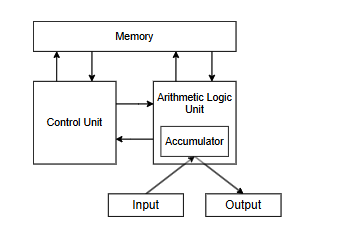
\includegraphics[width=0.6\linewidth]{asset/image1.png}
            \caption{Diagram Arsitektur Von Neumann}
            \label{fig:Arsitektur-Von-Neumann}
        \end{figure}

    
    \item Arsitektur Harvard

        \noindent
        \begin{figure}[H]
            \centering
            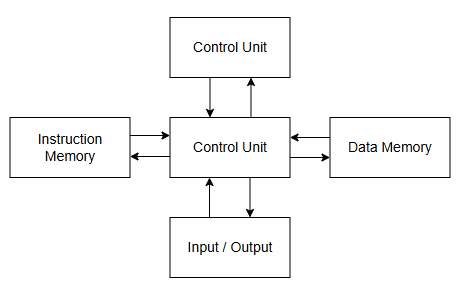
\includegraphics[width=0.6\linewidth]{asset/image2.png}
            \caption{Diagram Arsitektur Harvard}
            \label{fig:Diagram-Arsitektur-Harvard}
        \end{figure}
    


    \item Arsitektur ISA \textit{(Instruction Set Architecture)}

        \noindent
        \begin{figure}[H]
            \centering
            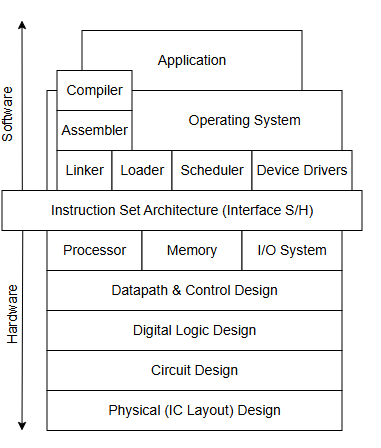
\includegraphics[width=0.3\linewidth]{asset/image3.png}
            \caption{Diagram Arsitektur ISA}
            \label{fig:Diagram-Arsitektur-ISA}
        \end{figure}

    

    
    \item Arsitektur Mikro

        \noindent
        \begin{figure}[H]
            \centering
            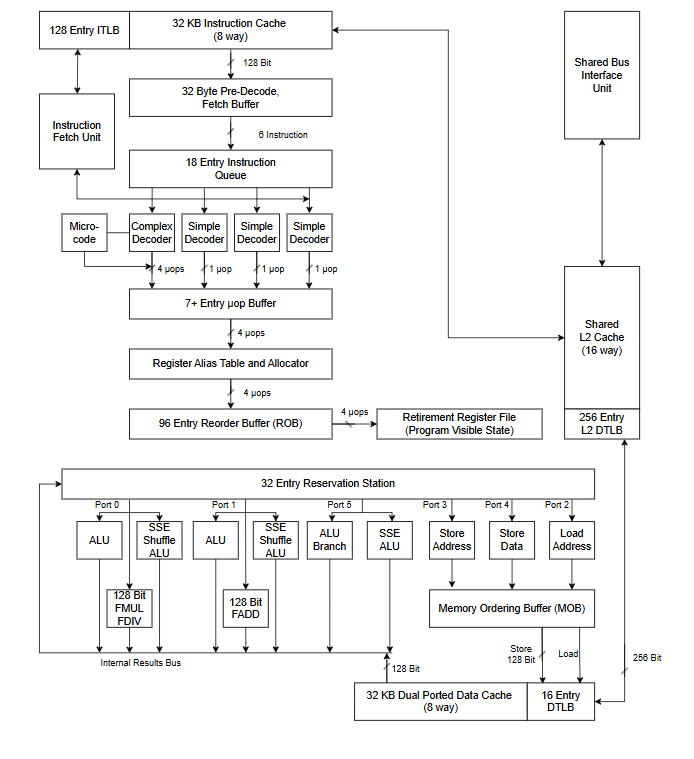
\includegraphics[width=0.4\linewidth]{asset/image4.png}
            \caption{Diagram Arsitektur Mikro}
            \label{fig:Diagram-Arsitektur-Mikro}
        \end{figure}
    

    \item Desain Sistem

      Desain sistem adalah proses yang melibatkan pembuatan kerangka kerja atau blueprint dari suatu sistem yang akan dibangun. Pada dasarnya, desain sistem bertujuan untuk menggabungkan berbagai elemen atau komponen yang ada dalam suatu sistem menjadi satu kesatuan yang berfungsi secara utuh dan terintegrasi. Desain ini memastikan bahwa semua komponen bekerja bersama untuk mencapai tujuan sistem secara efektif dan efisien. Dalam konteks sistem komputer, desain sistem meliputi perencanaan dan pengorganisasian elemen-elemen seperti CPU, memori, I/O \textit{(Input/Output)}, dan \textit{bus}.

      \item Arsitektur SISD \textit{(Single Instruction, Single Data)}


        \noindent
        \begin{figure}[H]
            \centering
            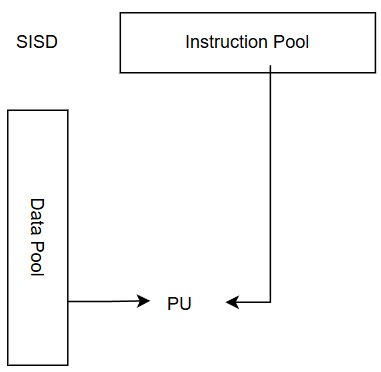
\includegraphics[width=0.4\linewidth]{asset/image6.png}
            \caption{Diagram Arsitektur SISD}
            \label{fig:Diagram-Arsitektur-SISD}
        \end{figure}
        
      
      Sistem Single Instruction Single Data (SISD) adalah arsitektur komputasi di mana satu instruksi diproses pada satu aliran data secara berurutan dalam sebuah mesin uniprosesor. CPU hanya menangani satu aliran instruksi dan satu aliran data pada satu waktu, menjadikannya ideal untuk komputasi sekuensial dalam sistem yang sederhana. Dalam sistem ini, instruksi dan data disimpan di memori utama, tetapi kecepatan pemrosesannya dibatasi oleh kecepatan transfer data internal. Model ini kurang cocok untuk aplikasi yang membutuhkan pemrosesan paralel atau kinerja komputasi tinggi.

    \begin{itemize}
        \item  Keuntungan  SISD adalah kesederhanaannya dan mudah diimplementasikan, cocok untuk komputasi sekuensial
        \item kekurangannya adalah tidak mendukung pemrosesan paralel, sehingga kinerjanya terbatas untuk tugas komputasi intensif atau modern yang membutuhkan pemrosesan simultan.
    \end{itemize}
    
    \item Arsitektur SIMD \textit{(Single Instruction, Multiple Data)}

        \noindent
        \begin{figure}[H]
            \centering
            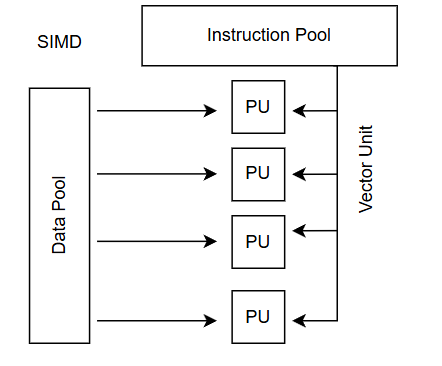
\includegraphics[width=0.4\linewidth]{asset/image7.png}
            \caption{Diagram Arsitektur SIMD}
            \label{fig:Diagram-Arsitektur-SIMD}
        \end{figure}
    
    Kelas komputer paralel dalam taksonomi Flynn. Ini menggambarkan komputer dengan beberapa elemen pemrosesan yang melakukan operasi yang sama pada beberapa titik data secara bersamaan. Dengan demikian, mesin tersebut memanfaatkan data tingkat paralelisme. SIMD ini terutama berlaku untuk tugas umum seperti menyesuaikan kontras dalam citra digital atau menyesuaikan volume audio digital. Paling modern CPU desain termasuk instruksi SIMD dalam rangka meningkatkan kinerja multimedia digunakan.

    \begin{itemize}
        \item Keuntungan utama sistem SIMD adalah kemampuannya untuk memproses banyak data sekaligus dengan satu instruksi. Misalnya, jika SIMD memuat delapan data sekaligus, operasi seperti add dapat diterapkan ke seluruh data dalam satu waktu, meningkatkan paralelisme dan efisiensi dibandingkan prosesor super-skalar
        \item kekurangannya adalah tidak semua algoritma, terutama yang berbasis aliran kontrol, dapat dioptimalkan dengan SIMD. Selain itu, kebutuhan register besar meningkatkan konsumsi daya, dan sebagian besar kompiler tidak secara otomatis menghasilkan instruksi SIMD, sehingga memerlukan tenaga ahli untuk implementasinya.
    \end{itemize}

    \item Arsitektur MISD \textit{(Multiple Instruction, Single Data)}

        \noindent
        \begin{figure}[H]
            \centering
            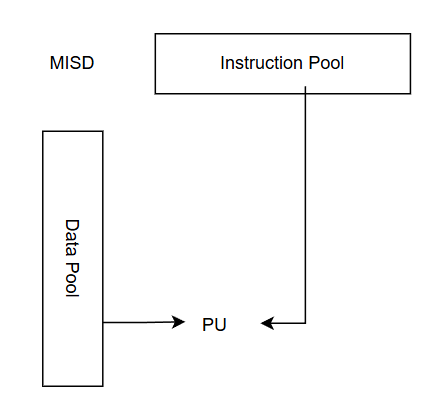
\includegraphics[width=0.4\linewidth]{asset/image8.png}
            \caption{Diagram Arsitektur MISD}
            \label{fig:Diagram-Arsitektur-MISD}
        \end{figure}

    MISD \textit{(Multiple Instruction, Single Data)} adalah jenis arsitektur komputasi paralel di mana beberapa prosesor menjalankan operasi berbeda pada data yang sama secara bersamaan. Arsitektur ini digunakan untuk mendeteksi dan menutupi kesalahan, seperti pada sistem toleransi kesalahan yang menggunakan replikasi tugas untuk memastikan keandalan. Meskipun termasuk dalam jenis komputasi paralel, MISD kurang umum dibandingkan dengan arsitektur SIMD dan MIMD, yang lebih cocok untuk pemrosesan data paralel pada umumnya. Contoh penerapannya jarang, karena efisiensinya yang lebih rendah dibanding arsitektur lainnya.

    \begin{itemize}
        \item keuntungan MISD dalam deteksi kesalahan dan peningkatan keamanan karena beberapa prosesor menjalankan instruksi berbeda pada data yang sama, memungkinkan validasi hasil secara efektif. Sistem ini ideal untuk aplikasi yang memerlukan keandalan tinggi, seperti toleransi kesalahan.
        \item kekurangannya adalah penggunaan yang sangat terbatas dalam komputasi umum, karena tidak efisien untuk tugas-tugas yang memerlukan paralelisme standar. kekurangannya adalah penggunaan yang sangat terbatas dalam komputasi umum, karena tidak efisien untuk tugas-tugas yang memerlukan paralelisme standar. 
    \end{itemize}
    \item Arsitektur MIMD \textit{(Multiple Instruction, Multiple Data)}

        \noindent
        \begin{figure}[H]
            \centering
            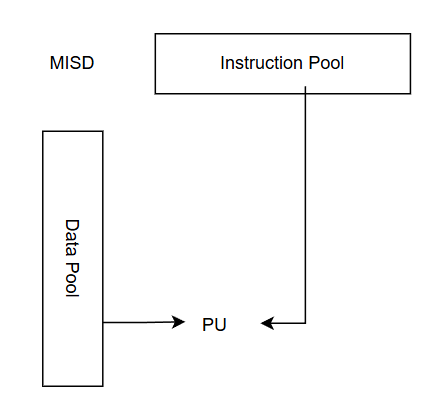
\includegraphics[width=0.4\linewidth]{asset/image8.png}
            \caption{Diagram Arsitektur MIMD}
            \label{fig:Diagram-Arsitektur-MIMD}
        \end{figure}
        
    MIMD \textit{(Multiple Instruction Multiple Data)} adalah arsitektur di mana beberapa instruksi dapat dieksekusi secara paralel pada banyak unit data. Dengan kata lain, MIMD menerapkan berbagai instruksi pada beberapa data secara bersamaan. Arsitektur ini menggunakan mekanisme sinkronisasi lokal yang eksplisit, yang membuatnya fleksibel, tetapi juga menyebabkan perangkat lunak menjadi lebih kompleks karena programmer atau kompiler paralelisasi harus menulis secara langsung perintah untuk komunikasi data antara prosesor yang berbeda.

    \begin{itemize}
    
        \item keuntungan arsitektur MIMD seperti fleksibilitas tinggi, skalabilitas, dan kecocokan untuk berbagai aplikasi karena mampu menjalankan instruksi yang berbeda secara paralel.

        \item kekurangan arsitektur MIMD adalah kompleksitas dalam desain perangkat keras dan pemrograman, serta efisiensi yang sangat bergantung pada pengaturan beban kerja, yang bisa membuatnya kurang optimal jika tidak dikelola dengan baik.
    \end{itemize}
\end{enumerate}

\begin{thebibliography}{9} 

\bibitem{SISD} ScienceDirect. (n.d.). \textit{Single Instruction Single Data (SISD)}. Retrieved October 3, 2024, https://www.sciencedirect.com/topics/computer-science/single-instruction-single-data

\bibitem{Kahfie2024} Kahfie, M. (2024). Tugas 4 Arsitektur SIMD dan SISD. Retrieved October 3, 2024, https://kahfie.com/tugas-4-arsitektur-simd-dan-sisd
.

\end{thebibliography}

\subsection{Process Description and Control}
Processes are a central concept in operating systems. This section covers:
\begin{itemize}
    \item Process states and state transitions
    \item Process control block (PCB)
    \item Context switching
\end{itemize}

\subsection{Scheduling Algorithms}
This section covers:
\begin{itemize}
    \item First-Come, First-Served (FCFS)
    \item Shortest Job Next (SJN)
    \item Round Robin (RR)
\end{itemize}
It explains how these algorithms are used to allocate CPU time to processes.

\subsection{Process Creation and Termination}
Details how processes are created and terminated by the operating system, including:
\begin{itemize}
    \item Process spawning
    \item Process termination conditions
\end{itemize}

\subsection{Introduction to Threads}
This section introduces the concept of threads and their relation to processes, covering:
\begin{itemize}
    \item Single-threaded vs. multi-threaded processes
    \item Benefits of multithreading
\end{itemize}

\begin{figure}[h]
    \centering
    % 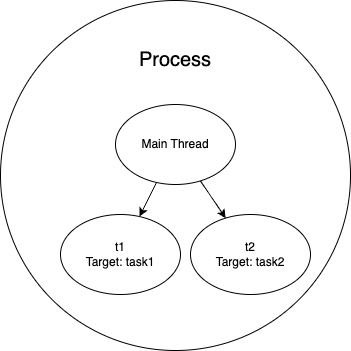
\includegraphics[width=0.5\textwidth]{/Users/khawaritzmi/Unhas/os_report_mid2024/a_class/asset/example.png}  % Sesuaikan nama file dan ukurannya
    \caption{Ini adalah gambar contoh dari multithreading.}
    \label{fig:contoh_gambar}
\end{figure}

Seperti yang terlihat pada Gambar \ref{fig:contoh_gambar}, inilah cara menambahkan gambar dengan keterangan.

\subsection{File Systems}
File systems provide a way for the operating system to store, retrieve, and manage data. This section explains:
\begin{itemize}
    \item File system structure
    \item File access methods
    \item Directory management
\end{itemize}

\subsection{Input and Output Management}
Input and output management is key for handling the interaction between the system and external devices. This section includes:
\begin{itemize}
    \item Device drivers
    \item I/O scheduling
\end{itemize}

\subsection{Deadlock Introduction and Prevention}
Explores the concept of deadlocks and methods for preventing them:
\begin{itemize}
    \item Deadlock conditions
    \item Deadlock prevention techniques
\end{itemize}

\subsection{User Interface Management}
This section discusses the role of the operating system in managing the user interface. Topics covered include:
\begin{itemize}
    \item Graphical User Interface (GUI)
    \item Command-Line Interface (CLI)
    \item Interaction between the user and the operating system
\end{itemize}

\subsection{Virtualization in Operating Systems}
Virtualization allows multiple operating systems to run concurrently on a single physical machine. This section explores:
\begin{itemize}
    \item Concept of virtualization
    \item Hypervisors and their types
    \item Benefits of virtualization in modern computing
\end{itemize}

\section{Assignments and Practical Work}
\subsection{Assignment 1: Process Scheduling}
Students were tasked with implementing various process scheduling algorithms (e.g., FCFS, SJN, and RR) and comparing their performance under different conditions.
\subsubsection{Group 1}
\begin{python}
    class Process:
    def __init__(self, pid, arrival_time, burst_time):
        self.pid = pid
        self.arrival_time = arrival_time
        self.burst_time = burst_time
        self.completion_time = 0
        self.turnaround_time = 0
        self.waiting_time = 0
\end{python}

\begin{table}[htbp] % Optional: For floating position
    \centering
    \begin{tabular}{|c|c|c|} % Defines number of columns and alignment (c = center, l = left, r = right). '|' creates vertical lines.
    \hline
    Header 1 & Header 2 & Header 3 \\ % Column headers
    \hline
    Row 1, Column 1 & Row 1, Column 2 & Row 1, Column 3 \\ % First row of data
    \hline
    Row 2, Column 1 & Row 2, Column 2 & Row 2, Column 3 \\ % Second row of data
    \hline
    \end{tabular}
    \caption{Your table caption} % Optional: For adding a caption
    \label{tab:your_label} % Optional: For cross-referencing the table
\end{table}
\subsection{Assignment 2: Deadlock Handling}
In this assignment, students were asked to simulate different deadlock scenarios and explore various prevention methods.

\subsection{Assignment 3: Multithreading and Amdahl's Law}
This assignment involved designing a multithreading scenario to solve a computationally intensive problem. Students then applied **Amdahl's Law** to calculate the theoretical speedup of the program as the number of threads increased.

\subsection{Assignment 4: Simple Command-Line Interface (CLI) for User Interface Management}
Students were tasked with creating a simple **CLI** for user interface management. The CLI should support basic commands such as file manipulation (creating, listing, and deleting files), process management, and system status reporting.

\subsection{Assignment 5: File System Access}
In this assignment, students implemented file system access routines, including:
\begin{itemize}
    \item File creation and deletion
    \item Reading from and writing to files
    \item Navigating directories and managing file permissions
\end{itemize}

\section{Conclusion}
The first half of the course introduced core operating system concepts, including process management, scheduling, multithreading, and file system access. These topics provided a foundation for more advanced topics to be covered in the second half of the course.

\end{document}